\section{Compression Optimal Algorithms}
\label{sec-optimal}

This section reviews the compression optimal \lsa algorithms find the minimum number of points or segments to represent the original trajectory \wrt an error bound $\epsilon$.

The naive optimal algorithm (\opt) \cite{Imai:Optimal} first formulates the \emph{min-$\#$} problem as a graph reachability problem, and solves the problem in  $O(n^3)$ time, where $n$ is the number of the original points of a trajectory. It is initially designed to support \ped, but can easily be modified to support \sed and \dad.
By using \textit{convex hull} \cite{Toussaint:Optimal} and \textit{sector intersection} \cite{Melkman:Optimal}, faster optimal algorithms are proposed with an improved time complexity to $O(n^2 \log n)$. Further, \cite{Chan:Optimal} \textcolor{blue}{proves the \emph{min-$\#$} problem (using \ped) for a general polygonal curve can be solved in $O(n^2)$ time by using the \textit{sector intersection} mechanism, and for some special curve, either open or closed (if there is an edge joining the first and the last points, then it is closed; otherwise, it is open) polygonal curve that forms part of a convex polygon, this problem can be solved in $O(n)$ time. Note that, in general, a trajectory is not necessary a convex or closed polygonal curve, instead, it is often open and concave. Thus, the best optimal algorithm for trajectory simplification using \ped still has $O(n^2)$ time.} 
%
\textcolor{blue}{\optss~\cite{Chen:Fast} using \lissed also has a time complexity of $O(n^2)$, and}
%
algorithm \kw{SP} \cite{Long:Direction} is essentially an optimization of the original optimal algorithm using \dad that achieves $O(n^2)$ time. 
%
However, all the above optimization mechanisms do not support \sed directly, and \opt remains the best optimal solution for \sed . {\em As all the optimized algorithms have the same effectiveness using the same distance metric, and essentially work for small size trajectories only, we choose algorithm \opt that supports \ped, \sed and \dad \myblue{(other optimal algorithms are not)} as the representative of optimal \lsa algorithms}.


%However, we argue that an optimal and a near optimal \lsa algorithms using \sed can achieve $O(n^2 \log n)$ time and $O(n^2)$ time, respectively, by applying the spatio-temporal cone intersection mechanism shown in Section~\ref{sec-cised} developed in our preview work \cised~\cite{Lin:Cised}.

%we introduce the naive optimal algorithm (\opt) \cite{Imai:Optimal} that runs in $O(n^3)$ time.
%The above optimized algorithms have the same effectiveness with the naive optimized algorithm using the same distance metric, thus, we won't go into them in detail.
%We then review a \ped specific optimal algorithm \optp \cite{Chan:Optimal} that achieves $O(n^2)$ time.
%Algorithms \opt and \optp are both evaluated in our experiments.
%Algorithm \opt is evaluated in our experiments.

%\subsection{The Naive Optimal Algorithm}
Given a trajectory \trajec{T}${[P_0, \ldots, P_n]}$ and an error bound $\epsilon$, algorithm \opt \cite{Imai:Optimal} solves the optimal trajectory simplification problem  in two steps: (1) it first constructs a reachability graph $G$ of \trajec{T}, and then (2) searches a shortest path from point $P_0$ to point $P_{n}$ in graph $G$.
%
The reachability graph of a trajectory \trajec{T}${[P_0, \ldots, P_n]}$ \wrt an error bound $\epsilon$ is $G$ = ($V$, $E)$, where (1) $V = \{P_0, \ldots, P_n\}$, and (2) for any nodes $P_s$ and $P_{s+k} \in V$ ($s\ge 0, k>0, s+k\le n$), edge $(P_s, P_{s+k}) \in E$ if and only if the distance of each point $P_{s+i} (0<i<k)$ to line segment $\vv{P_sP_{s+k}}$ is not greater than $\epsilon$.
%
Observe that in the graph $G$, (1) a path from nodes $P_0$ to $P_{n}$ is a representation of trajectory \trajec{T}. The path also reveals the subset of points of \trajec{T} used in the approximate trajectory, (2) the path length corresponds to the number of line segments in the approximate trajectory, and
(3) a shortest path is an optimal representation of trajectory \trajec{T}.

A straightforward way of constructing the reachability graph $G$ needs to check for all pairs of points $P_s$ and $P_{s+k}$ whether the distances of all points ($P_{s+i}$, $0<i<k$) to the line segment $\vv{P_sP_{s+k}}$ are less than $\epsilon$.
There are $O(n^2)$ pairs of points in the trajectory and checking the errors of all points $P_{s+i}$ to a line segment $\vv{P_sP_{s+k}}$ takes $O(n)$ time.
Thus, the construction step takes $O(n^3)$ time.
Finding a shortest path takes no more than $O(n^2)$ time. Hence, the straightforward algorithm, \ie~\opt, takes $O(n^3)$ time in total.
For space complexity, it needs $O(n^2)$ space.
%
Though the algorithm is initially developed using \ped, it is easy to see that it also supports \sed and \dad.


\begin{example}
	\label{exm-alg-optimal}
	Figure~\ref{fig:optimal} is an example of the \opt algorithm using \ped taking as input the trajectory \trajec{T} shown in Figure~\ref{fig:dp}. The reachability graph of \trajec{T} is constructed and a shortest path with 2 edges is founded.
	At last, the algorithm outputs two line segments $\vv{P_0P_4}$ and $\vv{P_4P_{10}}$.	
\end{example}
\vspace{-1ex}

\begin{figure}[tb!]
	\centering
	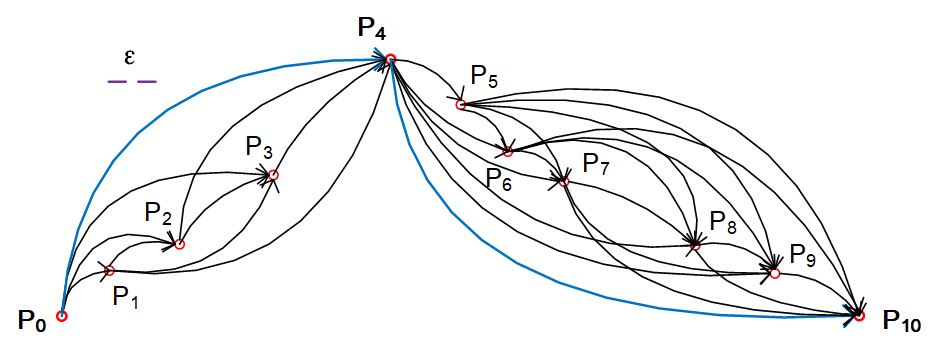
\includegraphics[scale=0.75]{Figures/Fig-Optimal.jpg}\vspace{-1ex}
	\caption{\small Example of reachability graph of trajectory \trajec{T}$[P_0, \ldots, P_n]$ whose shortest path is $(P_0, P_4, P_{10})$.}	\vspace{-3ex}
	\label{fig:optimal}
\end{figure}








\eat{%%%%%%%%%%%%%%%%%%%%%%%%20180722
\subsection{The Fast Optimal Algorithm Using \ped}
\label{subsec-optped}

Authors of \cite{Chan:Optimal} provide an optimal algorithm using \ped (\optp) that constructs the graph $G$ in $O(n^2)$ time, by using the \textit{sector intersection}\cite{Williams:Longest, Sklansky:Cone, Dunham:Cone, Zhao:Sleeve} mechanism.

For the start data point $P_s$, any point $P_{s+i}$ and $|\vv{P_sP_{s+i}}|>\epsilon$ ($i\in[1, k]$), there are two directed lines $\vv{P_sP^u_{s+i}}$ and $\vv{P_sP^l_{s+i}}$ such that $ped(P_{s+i}, \vv{P_sP^u_{s+i}})$ $=$ $ped(P_{s+i}, \vv{P_sP^l_{s+i}}) = \epsilon$ and either ($\vv{P_sP^l_{s+i}}.\theta < \vv{P_sP^u_{s+i}}.\theta ~and~\vv{P_sP^u_{s+i}}.\theta - \vv{P_sP^l_{s+i}}.\theta <\pi$) or ($\vv{P_sP^l_{s+i}}.\theta > \vv{P_sP^u_{s+i}}.\theta ~and~ \vv{P_sP^u_{s+i}}.\theta - \vv{P_sP^l_{s+i}}.\theta < -\pi)$. Indeed, they forms a \emph{sector} \sector{(P_s, P_{s+i}, \epsilon)} that takes $P_s$ as the center point and $\vv{P_sP^u_{s+i}}$ and $\vv{P_sP^l_{s+i}}$ as the border lines.


Then, given a point $P_s$, $0 \le s < n$, algorithm \optp builds a sector taking $P_s$ as the start point and checks for all points $P_{s+k}$, $k>0 ~and~ s+k \le n$, whether edge $(P_s, P_k)$ can be included in graph $G$. It can be added to the graph if and only if $(\bigsqcap_{i=1}^{k-1}\mathcal{S}(P_s, P_{s+i}, \epsilon)) \bigsqcap \vv{P_sP_{s+k}} \ne \{P_s\}$, \ie line segment $\vv{P_sP_{s+k}}$ ~passing through the common intersection area of sectors $\mathcal{S}(P_s, P_{s+i}, \epsilon))$, $0<i<k$.

There are $n$ points of $P_s$ in the trajectory and the checking of $(\bigsqcap_{i=1}^{k-1}\mathcal{S}(P_s, P_{s+i}, \epsilon)) \bigsqcap \vv{P_sP_{s+k}} \ne \{P_s\}$ for one $P_s$ takes $O(n)$ time.
Thus, the construction step takes $O(n^2)$ time and the algorithm takes $O(n^2)$ time in total.
For space complexity, this algorithm takes $O(n^2)$ space. However, it could be optimized to $O(n)$ space by the approach presented in \cite{Chen:Space}, whose fundamental idea is that it computes a shortest path in graph $G$ without having to maintain $G$ explicitly.

Algorithm \optp does not support \sed.


\begin{example}
	\label{exm-alg-optped}
	Figure~\ref{fig:optped} is a example of algorithm {\optp} taking as input the same trajectory $\dddot{\mathcal{T}}[P_0, \ldots, P_{10}]$. At the beginning, $P_0$ is the first start point, and points after $P_0$, \ie $P_1$, $P_2$, $P_3$, etc., each has a \emph{sector}. For example, the \emph{sector} $\mathcal{S}$($P_0$, $P_{2}$, $\epsilon$) takes $P_0$ as the center point and $\vv{P_0P^u_{2}}$ and $\vv{P_0P^l_{2}}$ as the border lines.
	Then, (1) for point $P_1$, edge $(P_0, P_1)$ is sure added to the graph $G$;
	(2) for point $P_2$, because $\bigsqcap_{i=1}^{2}\mathcal{S}(P_0, P_{0+i}, \epsilon) \ne \{P_0\}$ and $P_2$ is in the intersection area, edge $(P_0, P_2)$ is added to the graph $G$;
	(3) for points $P_3$ and $P_4$, edges $(P_0, P_3)$ and $(P_0, P_4)$ are added to the graph $G$ in turn;
	(4) for point $P_5$, because $P_5$ is NOT in the intersection area, edge $(P_0, P_5)$ should not be added to the graph $G$.
	After all edges start from $P_0$ have been checked, the process goes to the next step that takes $P_1$ as the new start point, and the process repeats.
	At last, the algorithm builds the same graph $G$ as shown in Figure~\ref{fig:optimal}, and outputs two line segments $\vv{P_0P_4}$ and $\vv{P_4P_{10}}$.
\end{example}

\begin{figure}[tb!]
	\centering
	\hspace{-1ex}\includegraphics[scale=0.66]{Figures/Fig-OptPed.jpg}\vspace{-3ex}
	\caption{\small The trajectory $\dddot{\mathcal{T}}$ is compressed by the fast optimal algorithm using \ped to two line segments.}	\vspace{-3ex}
	\label{fig:optped}
\end{figure}

}

\eat{%%%%%%%%%%%%%%%%%%%%%%%%%%%%%%%%%%%%%%%
\subsection{The Optimal Algorithm using \sed}
The constructing of the reachability graph $G$ using \sed can be optimized, by using the \textit{spatio-temporal cone intersection} mechanism (See Section~\ref{sec-siped}).

Given a point $P_s$, $0 \le s < n$, the optimal builds a cone taking $P_s$ as the start point and checks for all points $P_{s+k}$, $k>0 ~and~ s+k \le n$, whether $(P_s, P_k)$ can be included in graph $G$ by checking $(\bigsqcap_{i=1}^{k-1}\mathcal{C}(P_s, P_{s+i}, \epsilon)) \bigsqcap \vv{P_sP_{s+k}} \ne \{P_s\}$, \ie line segment $\vv{P_sP_{s+k}}$ ~passing through the common intersection area of cones $\mathcal{C}(P_s, P_{s+i}, \epsilon))$, $0<i<k$.

The checking of intersection of cones is equal to check the intersection of circles on a plane \cite{Lin:Cised}, which is claimed of $O(n \log n)$ time for $n$ circles~\cite{Shamos:Circle}.
There are $n$ points of $P_s$ in the trajectory and the checking for one $P_s$ takes $O(n \log n)$ time.
Thus, the construction step takes $O(n^2 \log n)$ time and the algorithm takes $O(n^2 \log n)$ time in total.

\stitle{Remark}.
If we approximate each circle by its $m$-edges inscribed regular polygon and approximate the intersection of $n$ circles on a plane by the intersection of their inscribed regular polygons, the way \cised does, then we get a near optimal graph $G'$ such that $\lim_{m \to \infty}{G'=G}$, and a \textit{near optimal} algorithm using \sed, \ie ~\nopts, that achieves $O(n^2)$ time. The space complexity of the near optimal algorithm also achieves $O(n)$ by combining the approach of \cite{Chen:Space}.
}
